\section{Methods}
\subsection{Framework and scope}\label{MainModelDescription}
We develop a probabilistic framework to examine how hurricane losses propagate through Florida's residential insurance system. We first estimate economic losses for each county and separate wind and flood contributions. We then allocate losses to private insurers, Citizens Property Insurance Corporation, the National Flood Insurance Program (NFIP), and those without sufficient insurance. Reinsurance and catastrophe bonds reimburse part of insurers' claims. The remaining claims draw on capital. When these resources are exhausted, assessments and federal borrowing provide further financing (Fig.~\ref{FigOverview}).

The financial model represents insurance market conditions in 2024. County exposure determines the initial allocation of losses, insurer balance sheets determine defaults, and statewide or national limits constrain the backstops. We evaluate individual storms, constructed sequences, and synthetic hurricane seasons. Future climate experiments retain the same market configuration to isolate the effect of changing hazards. They describe the stress that today's system would face under those conditions. Recovery and changes in the market across successive years are not modeled.

\begin{figure*}[htb!]
    \centering
    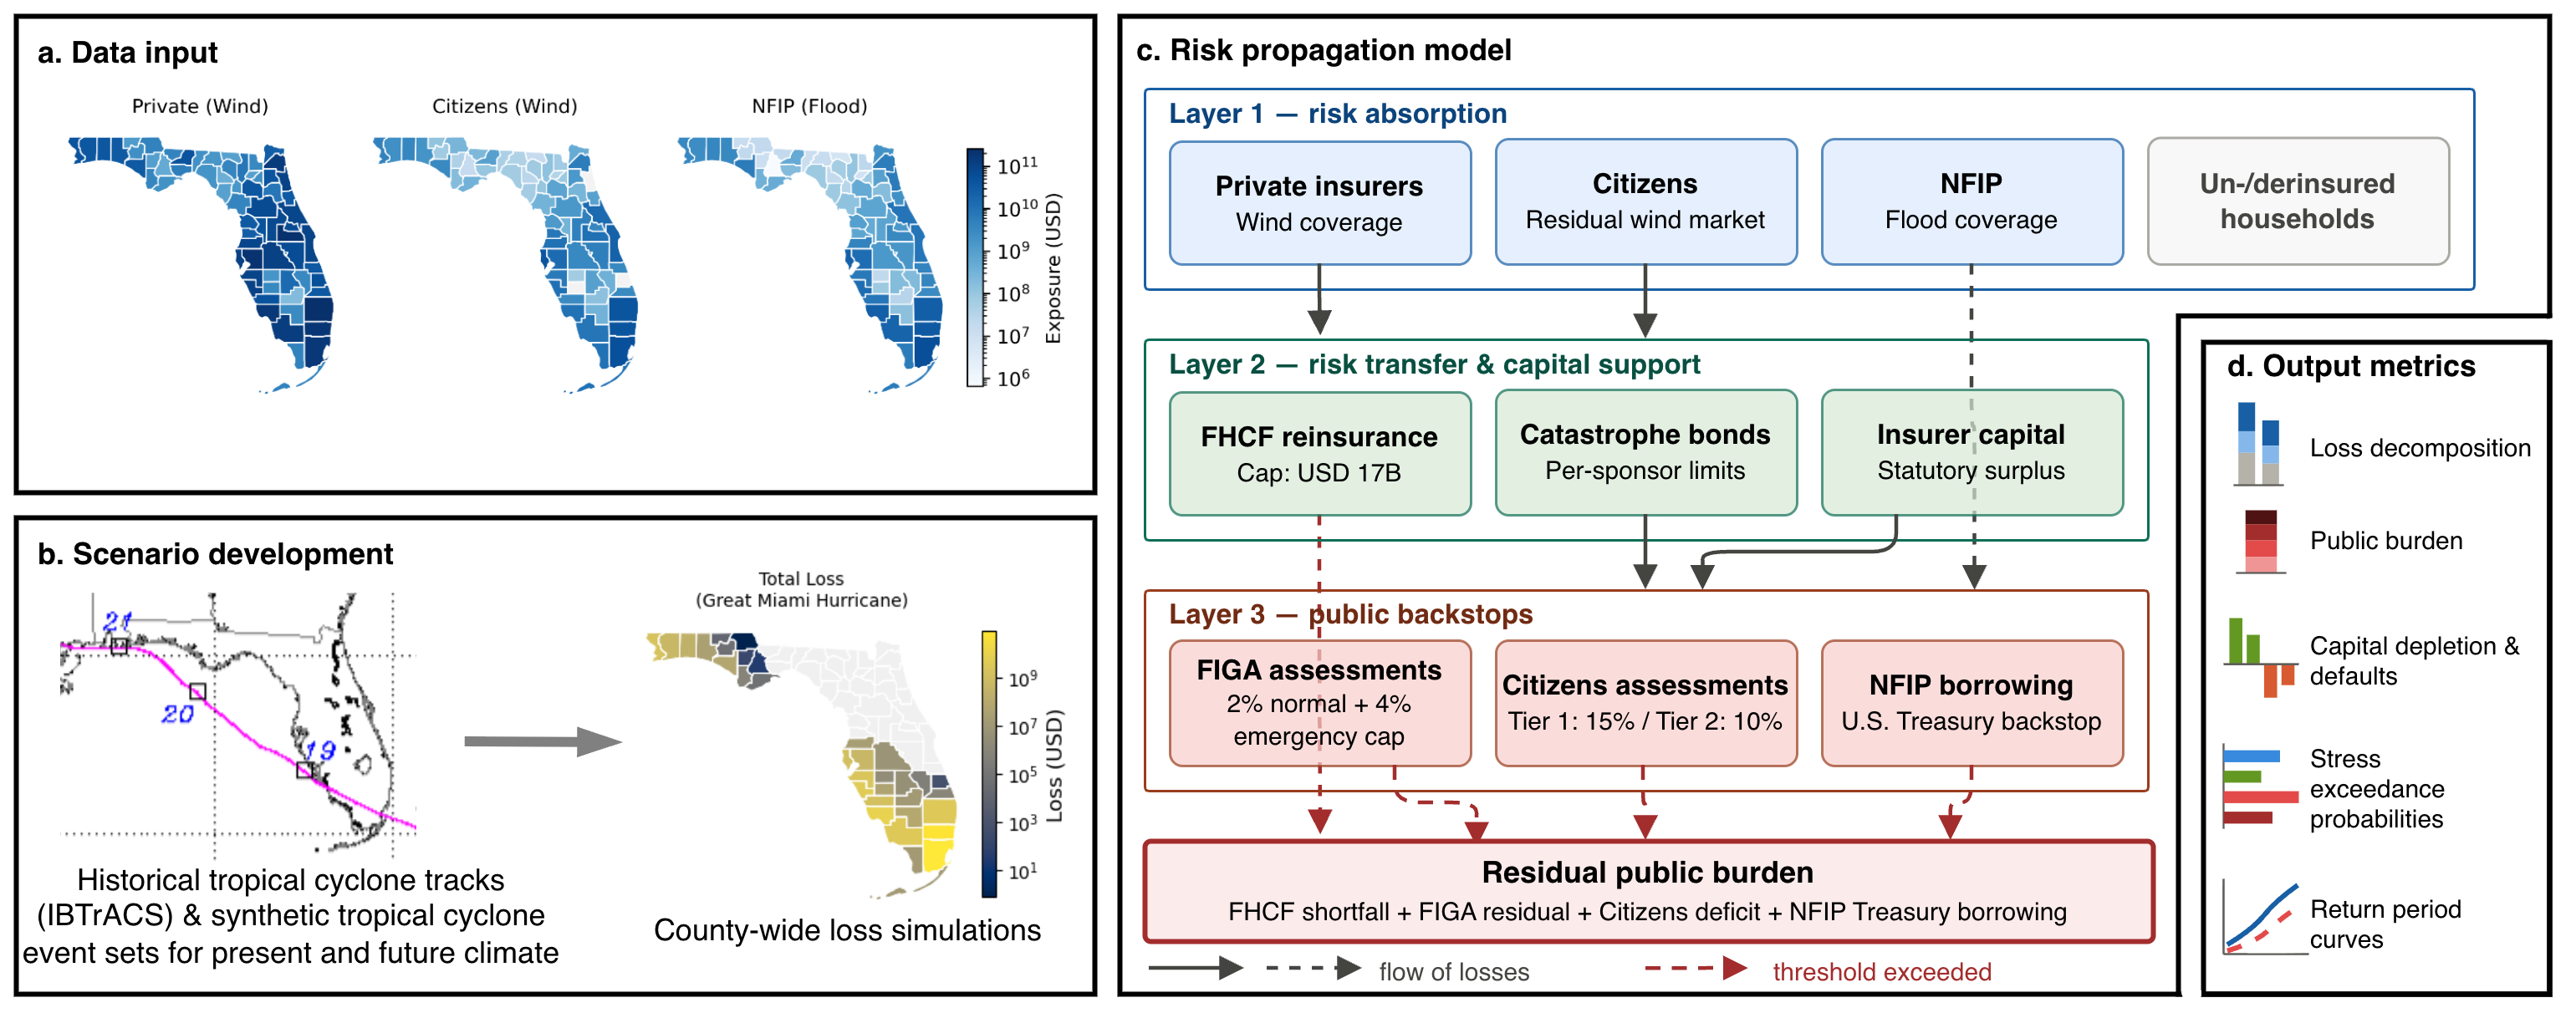
\includegraphics[width=1.0\textwidth]{figures/fig1_systemic_risk_overview_florida.png}
    \caption{\textbf{Insurance system architecture and risk propagation in the Florida homeowners' property insurance market.}
    a) County-level exposure and coverage-in-force for private wind insurers, Citizens Property Insurance Corporation (Citizens), and the U.S. National Flood Insurance Program (NFIP), together with the policy terms, capital positions, and contractual constraints used as model inputs.
    b) Illustrative example of the hazard-to-loss estimation for a single event. The track of the 1926 Great Miami Hurricane (from IBTrACS; left) is translated into county-level wind and flood loss estimates using the specified economic exposure (right). For clarity, only this one historical track is shown; the probabilistic analysis additionally draws on large synthetic tropical cyclone event sets representing present-day and future climate conditions (Methods), which are not displayed here.
    c) Loss propagation through three sequential layers. (1) risk absorption by private insurers, Citizens, the NFIP, and un-/under-insured households; (2) risk transfer and capital support via the Florida Hurricane Catastrophe Fund (FHCF; statewide seasonal cap USD 17B), catastrophe bonds, and insurer statutory surplus; and (3) public backstops, comprising Florida Insurance Guaranty Association (FIGA) assessments (2\% normal plus up to 4\% emergency), Citizens' two-tier assessments (Tier 1 up to 15\%, Tier 2 up to 10\%), and NFIP Treasury borrowing, which together determine the residual public burden. Solid arrows denote the flow of losses; dashed black arrows indicate the flow of losses that bypass one layer; dashed red arrows indicate losses transferred once an institutional threshold or statutory cap is exceeded.
    d) Main output metrics are color-coded to the model layer in (c) that generates them. They include loss decomposition, public burden by backstop, insurer capital depletion and defaults, stress exceedance probabilities, and return period curves, evaluated under single, sequential, and probabilistic event scenarios.}
    
\label{FigOverview}
\end{figure*}


\subsection{Hurricane hazards and economic losses}\label{DataTCtracks}\label{MethodsHazModel}\label{MethodsWindFloodSplit}
Historical tropical cyclone (TC) tracks come from IBTrACS \cite{knapp_international_2010}. Synthetic tracks are generated with the statistical-dynamical MIT TC model \cite{emanuel_statistical_2006,emanuel_hurricanes_2008}, using ERA5 for the present climate and five CMIP6 global climate models (GCMs) for future conditions. We retain tracks passing within 150~km of Florida's coast. The ERA5 reference spans 1980--2023. Each GCM supplies a historical reference for 1995--2014 and projections for 2041--2060 and 2081--2100. Track generation and frequency calibration are described in Supporting Text~S2.

We calculate economic losses with CLIMADA \cite{aznar-siguan_climada_2019}. The Holland wind model \cite{holland_revised_2008} converts each track into a wind field on a grid of 120~arc-seconds. LitPop distributes 2020 GDP values using population and nightlight intensity \cite{eberenz_asset_2020}. We combine this exposure with the USA impact function, which relates wind intensity to relative economic damage \cite{eberenz_regional_2021}. Although wind provides the predictor, the function was calibrated against total cyclone losses and incorporates average rainfall and surge contributions. It does not resolve damage to individual residential buildings. We aggregate the resulting losses to counties before applying the insurance model.

Wind and flood losses enter different insurance programs. To separate them, we use county contributions derived from the multi-hazard damage regression of Gori et al.\ \cite{gori_sensitivity_2025,gori_tropical_2025}. For each realization, we rescale these contributions to a sampled wind share, centered at 84.6\% for the synthetic catalog. Historical scenarios use separate wind share distributions. Flood loss is the remainder. This approach partitions aggregate economic losses rather than independently simulating rainfall and surge damage. Sea-level rise is not included. Supporting Text~S2 gives the attribution equations, rescaling procedure, and wind share means for historical storms.

\subsection{Insurance exposure and loss allocation}\label{DataInsuranceMarket}\label{MethodsRiskAbsorption}
We assign county wind exposure to private insurers and Citizens using their total insured values. Private exposure comes from Florida Hurricane Catastrophe Fund (FHCF) reports, and Citizens supplies its own county records \cite{fhcf_coverage_2024,citizens_policies_in_force_2024}. Within the private market, we allocate exposure among the largest 100 insurers in proportion to their statewide residential premiums \cite{floir_marketshare_2024}. Applying the same shares across counties preserves statewide market composition but removes differences in insurers' geographic concentration. Statutory surplus reported for individual insurers and affiliated groups, obtained through S\&P Capital IQ, defines available capital. Supporting Text~S1 documents these inputs and their reference dates.

We represent the insured share of wind losses with a Beta(4,6) distribution, with mean 0.40. Its calibration uses Florida insurance losses, NFIP payments, and reconstructed economic losses for 2017--2024 (Supporting Text~S3). The empirical ratio has total economic loss in its denominator, whereas the model applies the fraction to wind loss. We therefore use it as an allocation assumption, not a direct measurement of residential wind coverage. Insured wind losses are divided among insurers by county exposure. The remaining losses stay outside the modeled insurance system. These losses cannot be assigned entirely to households because the economic exposure includes more than residential property.

For flood, FEMA's NFIP Residential Penetration Rates dataset estimates the proportion of residential structures insured in each county \cite{fema_nfip_penetration_2025}. The denominator is the estimated residential stock from the National Structure Inventory. We combine rates inside and outside Special Flood Hazard Areas using their shares of that stock. We apply the resulting county rate to flood losses and cap claims at county NFIP coverage-in-force \cite{fema_nfip_redacted_policies_v2_2024}. This assumes that insured structures carry the same share of losses as their share of the county's residential stock. Supporting Text~S3 details the calculation and its limitations.

\subsection{Risk transfer, capital depletion, and institutional backstops}\label{MethodsRiskProp}\label{MethodsRiskTransferCapital}
The FHCF reimburses participating wind insurers for eligible claims above a retention, the amount they must first absorb themselves. Recoveries depend on each insurer's chosen reimbursement percentage and contract limit \cite{fhcf_annual_report_2023,fhcf_coverage_2024}. We constrain combined recoveries to the modeled seasonal capacity of USD~17~billion and reduce them proportionally when demand exceeds that amount. Catastrophe bonds provide additional recoveries when the relevant loss thresholds are reached, up to their payout limits \cite{artemis_catbond_2024}. We represent them as covers for a single occurrence without reinstatement. Private reinsurance treaties are not included.

We subtract recoveries from insured wind losses and apply the remaining claims to statutory surplus. An insurer with negative surplus may receive support from an affiliated group, subject to the group's available capital and an eligibility rule. Insurers still in deficit after this support are classified as insolvent. This calculation represents the exhaustion of modeled capital, rather than a prediction of a regulatory liquidation decision. Supporting Text~S4 specifies the contracts, capital accounting, and group support rule.

The Florida Insurance Guaranty Association (FIGA) covers claims following private insurer insolvency through assessments on surviving insurers. We compare the combined deficit with one year's modeled assessment capacity, comprising 2\% normal and 4\% emergency assessments of surviving insurers' written premiums \cite{flastat,figa_assessments}. Any excess remains a residual financing requirement. For Citizens, losses remaining after recoveries draw on its statutory surplus \cite{citizens_annual_statement_2024}. Two assessment tiers then provide financing, limited in the model to 15\% of Citizens' premium base and 10\% of the statewide property premium base \cite{citizens_assessments}. We record the deficit remaining after both tiers. These assessments spread costs among insurers and policyholders. They are not state expenditure. The calculation does not capitalize future assessment streams or represent financing through bonds backed by those streams.

NFIP claims draw on a national fund balance of USD~3.441~billion \cite{crs_nfip_fund_balance_2025}. Claims above this amount are recorded as Treasury borrowing requirements. We do not represent NFIP reinsurance or enforce the statutory borrowing ceiling. This output therefore measures the additional financing required under the modeled claims, including amounts that may exceed existing borrowing authority. Losses elsewhere in the United States are outside the analysis. Together, these rules identify where insured losses exceed available resources. The thresholds can cause residual requirements to rise faster than gross losses as additional financing layers are exhausted. Full equations and parameter values are provided in Supporting Text~S4 and Table~S9.

\subsection{Simulation design and experiments}\label{MethodsFutureClim}\label{MethodsPolicy}\label{MethodsBuildingCodeClimate}
We apply the model to four historical storm footprints and three constructed sequences, with 200 Monte Carlo realizations per scenario. These are stress tests under the specified exposure and market conditions, rather than reconstructions of historical losses. Sequential scenarios reduce exposed asset values after the first storm but do not model changes in vulnerability or recovery. The probabilistic assessment samples storms with replacement according to catalog frequencies to form 10,000 synthetic seasons for each climate dataset, including seasons with no events. We apply the financial model once to each season's aggregated losses, starting with the same capital in every season. Supporting Text~S5 describes the sampling and aggregation.

For SSP2--4.5, we estimate each GCM's change in a risk metric between its future and historical simulations. We add the median change across the five GCMs to the ERA5 baseline. This combines the baseline estimate with the modeled climate signal rather than using GCM projections directly as future risk levels. The same procedure applies to expected annual losses and exceedance probabilities. Additional scenario comparisons are documented in Supporting Text~S5.

We also vary market structure, insurance coverage, and physical losses in separate experiments. Market contraction increases Citizens' share from 15\% to 25\%, with changes in exposure and capital. Expanded coverage raises the assumed insured wind fraction from 40\% to 60\% and flood penetration from approximately 11\% to 30\%, alongside changes in premiums, capital, and Citizens' share. The mitigation experiment reduces wind losses by 30\% and flood losses by 25\% before insurance allocation. These prescribed reductions represent the effect of lower damage, not an engineering model of particular building standards. Finally, we vary loss reductions to identify those that offset mid-century climate effects on each metric. Supporting Text~S5 gives the scenario settings and the offset calculation.

\subsection{Outcome metrics and amplification}\label{MethodsOutput}
We track uninsured losses, insured claims, insurer defaults, and the largest insurer deficit. Institutional stress is measured against each modeled capacity. We also compare NFIP claims with Florida premium income and aggregate burden with Florida GDP. Table~S2 defines all indicators.

The public burden indicator combines FIGA and Citizens residual deficits and NFIP borrowing requirements. FHCF reimbursement shortfalls are tracked separately: tracing the model shows that whenever an FHCF shortfall is not absorbed by an insurer's own remaining capital, it already appears inside that insurer's or Citizens' deficit, so adding it to the sum would double-count that portion. The indicator records stress across financing channels whose costs need not fall on the same actors, and it should not be interpreted as a forecast of government expenditure.
% RESOLVED (Earth's Future revision, correction register item C1). Verified
% by tracing fl_risk_model.runner (capital depletion is applied to net wind
% loss, after FHCF and cat-bond recovery) and confirmed with deterministic
% fixtures (fl_risk_model/tests/earths_future/test_accounting_fixtures.py).

Annual exceedance probabilities are the fraction of simulated seasons above a specified threshold. Return periods express the inverse annual exceedance probability. In Table~\ref{TabProbRPvalues}, the public burden return levels are now the empirical quantiles of the season-level sum of its components, and total loss return levels remain independently ranked marginal quantiles. Figure~\ref{FigLossPublicBurdenScaling} compares these two series; it is not a claim about paired outcomes within individual seasons for the loss side, though the public burden series is now itself a genuine season-level aggregate. Supporting Text~S6 gives the estimator and the quantile convention.
% RESOLVED (correction register item R1). Table 1 and the amplification
% figure were recalculated from season-level sums using
% scripts/earths_future_revision/section5_return_periods.py on the archived
% ERA5 baseline (10,000 seasons); see the correction register for the
% numerical effect (10y/100y amplification: 43.9x submitted -> 31.1x
% corrected; power-law exponent 1.64 -> 1.51).

\subsection{Uncertainty and model evaluation}\label{MethodsUncertainty}
We sample the insured wind fraction, wind share, and county insured values, the latter with a coefficient of variation of 0.15. Other financial parameters remain fixed within each experiment. Table~S8 separates sampled inputs from fixed assumptions and climate model variation.

We examine sensitivity to the insured wind fraction over values from 0.1 to 0.5 (Table~S6) and to NFIP flood-loss allocation using three configurations that assign county flood losses through the baseline structure-weighted rate, entirely within Special Flood Hazard Areas, or entirely outside them (Supporting Text~S3). A 300-season by 50-parameter-draw nested design was also used to compare hazard-driven and parameter-driven variance; because the 300 seasons were selected to span the loss distribution rather than sampled at random, this design does not evaluate uncertainty in all structural assumptions and is not the basis for the robustness claims in this paper.

We use 1,000 bootstrap resamples of the ERA5 seasons to characterize sampling uncertainty. Future estimates additionally report the 10th to 90th percentile range of changes across GCMs. These ranges represent different sources of uncertainty. Comparisons with normalized historical losses and Florida's institutional experience provide consistency checks, rather than formal validation. In particular, the low modeled FHCF recovery for Irma reflects its assumed wind share and differs from observed reimbursements. Supporting Text~S6 describes the checks and their scope.
